\chapter{系统设计与实现}

\section{系统设计目标}

针对“三高”慢性病医学问答场景中信息专业性强、回答可靠性要求高以及实时交互需求明显的特点，本文设计并实现了一种基于检索增强生成的智能医学问答系统，在综合分析医学问答任务特点的基础上，设定了四个方面的设计目标。

第一个方面是准确性，医学问答系统首先要保证回答内容的科学性与准确性，因为医学知识具有高度专业性，错误或不严谨的信息可能对用户产生误导甚至带来潜在风险，为了应对这一问题，本系统构建了高质量的“三高”慢性病医学知识库，并采取关键词检索与语义向量检索相结合的混合检索策略，从权威资料中获取与用户问题高度相关的医学证据，再引入RAG机制，把检索到的证据作为约束条件输给大语言模型，从而有效抑制模型自行编造内容的幻觉现象，提升回答的事实一致性与专业可靠性。

第二个方面是可解释性，与通用问答系统不同，医学问答不仅需要给出结论，还要让用户能够理解答案的依据来源，为此本系统在生成回答的同时保留并展示相关的医学证据来源信息，比如指南或科普文章，通过展示“回答正文加上引用来源”的结构让用户能够追溯信息源头，同时在提示语设计中对模型输出施加结构化约束，促使生成内容尽可能围绕检索到的证据展开，进一步增强系统的可解释性。

第三个方面是实时性，在实际应用场景里用户通常期望快速获得问答结果，这就要求系统具备良好的响应速度，考虑到大语言模型推理的计算开销较大，本系统把大语言模型部署在高性能服务器上并引入多种性能优化策略，包括用向量检索来加速知识匹配过程、利用混合精度计算降低模型推理开销、以及通过键值缓存机制减少重复运算，从而显著提升生成效率，同时在系统架构层面采用前后端分离设计，使用户请求能被快速处理并返回结果，满足实时交互的需求。

第四个方面是可扩展性，随着医学知识的持续更新和应用需求的不断拓展，系统需要具备良好的扩展能力，一方面知识库设计采用模块化管理方式，支持医学数据的增删操作，便于持续纳入新的医学指南和研究成果，另一方面在系统架构上把知识库、检索模块与生成模型彼此之间保持松耦合关系，使各模块能独立升级或替换，比如可以在不影响整体系统结构的情况下更换更高性能的向量模型或大语言模型，从而保证系统在未来具备良好的演进能力与适应性。

\section{系统总体架构}

本系统整体架构采用分层式设计，将交互逻辑、业务逻辑、模型能力与数据能力进行划分，各模块之间相对独立，能够在一定程度上实现故障隔离。系统架构如图\ref{fig:framework-structure}所示，主要由四个层次构成。

前端应用层只承担交互和状态管理，不直接参与模型推理，具体包括用户登录、会话管理、消息渲染、流式展示、引用证据呈现以及管理员知识库入口等功能。

业务服务层基于Node.js，采用Express框架构建统一的 API 网关，用于对外提供服务接口。业务服务层主要负责身份认证与权限控制、会话上下文组织、消息持久化、模型服务编排和知识库维护。

模型推理层是一套独立的Python服务，部署在高性能GPU服务器上，基于Flask框架对外提供接口。该层主要负责向量数据库检索、相关文档重排序、提示词组装、模型推理及流式事件输出。模型服务对外暴露同步与流式两类接口，业务服务可以根据实际场景灵活选择调用方式。将推理服务独立部署后，可在不影响业务API的情况下单独升级模型和检索策略。

数据与索引层中使用关系型数据库保存用户、会话、消息与文档元数据；使用FAISS向量索引存储医学指南等医学资料，并将文本编码为向量构建索引结构以支持向量检索和BM25检索。

\vspace{10pt}
\begin{figure}[htb]
    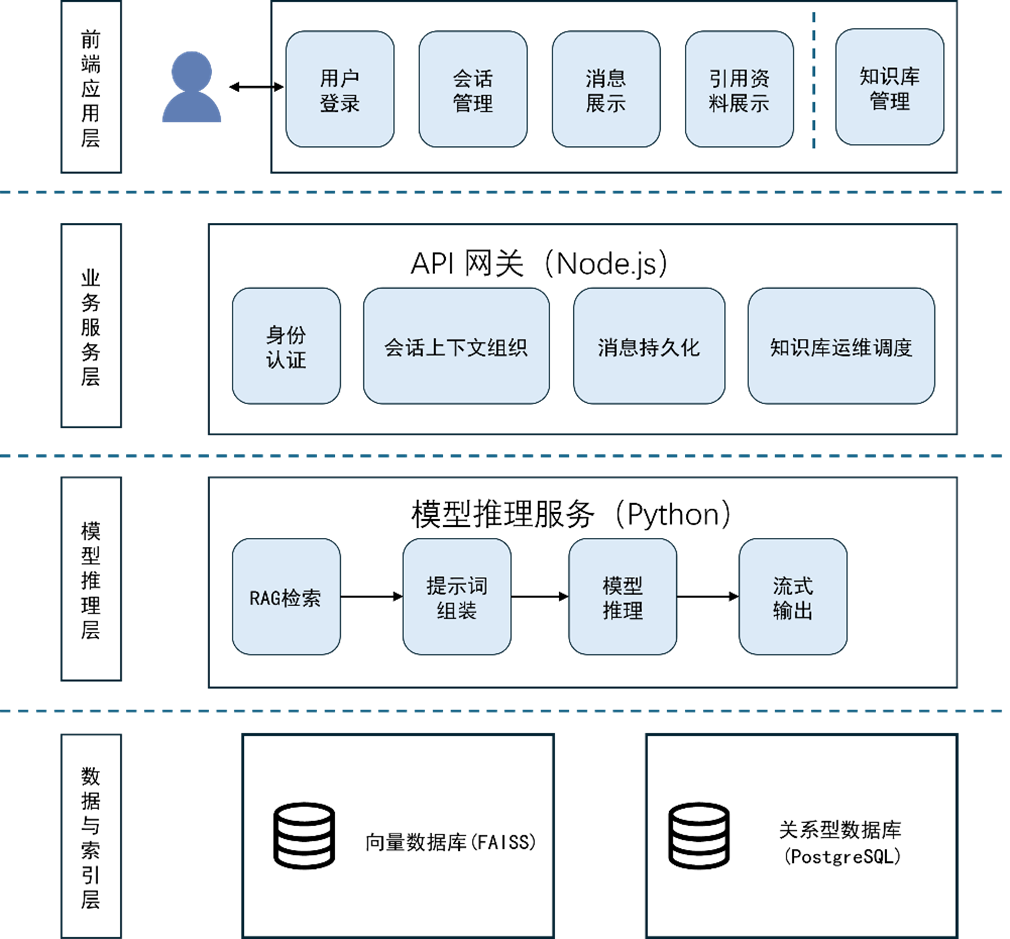
\includegraphics[width=0.8 \textwidth]{image/4/系统架构图.png}
    \caption{系统架构图}
    \label{fig:framework-structure}
\end{figure}

\section{系统流程设计}

针对“三高”慢病管理场景，本文将问答流程划分为“输入解析—知识检索—上下文增强—答案生成”四个阶段。系统流程如\ref{fig:system-flowchart}所示。

\vspace{10pt}
\begin{figure}[htb]
    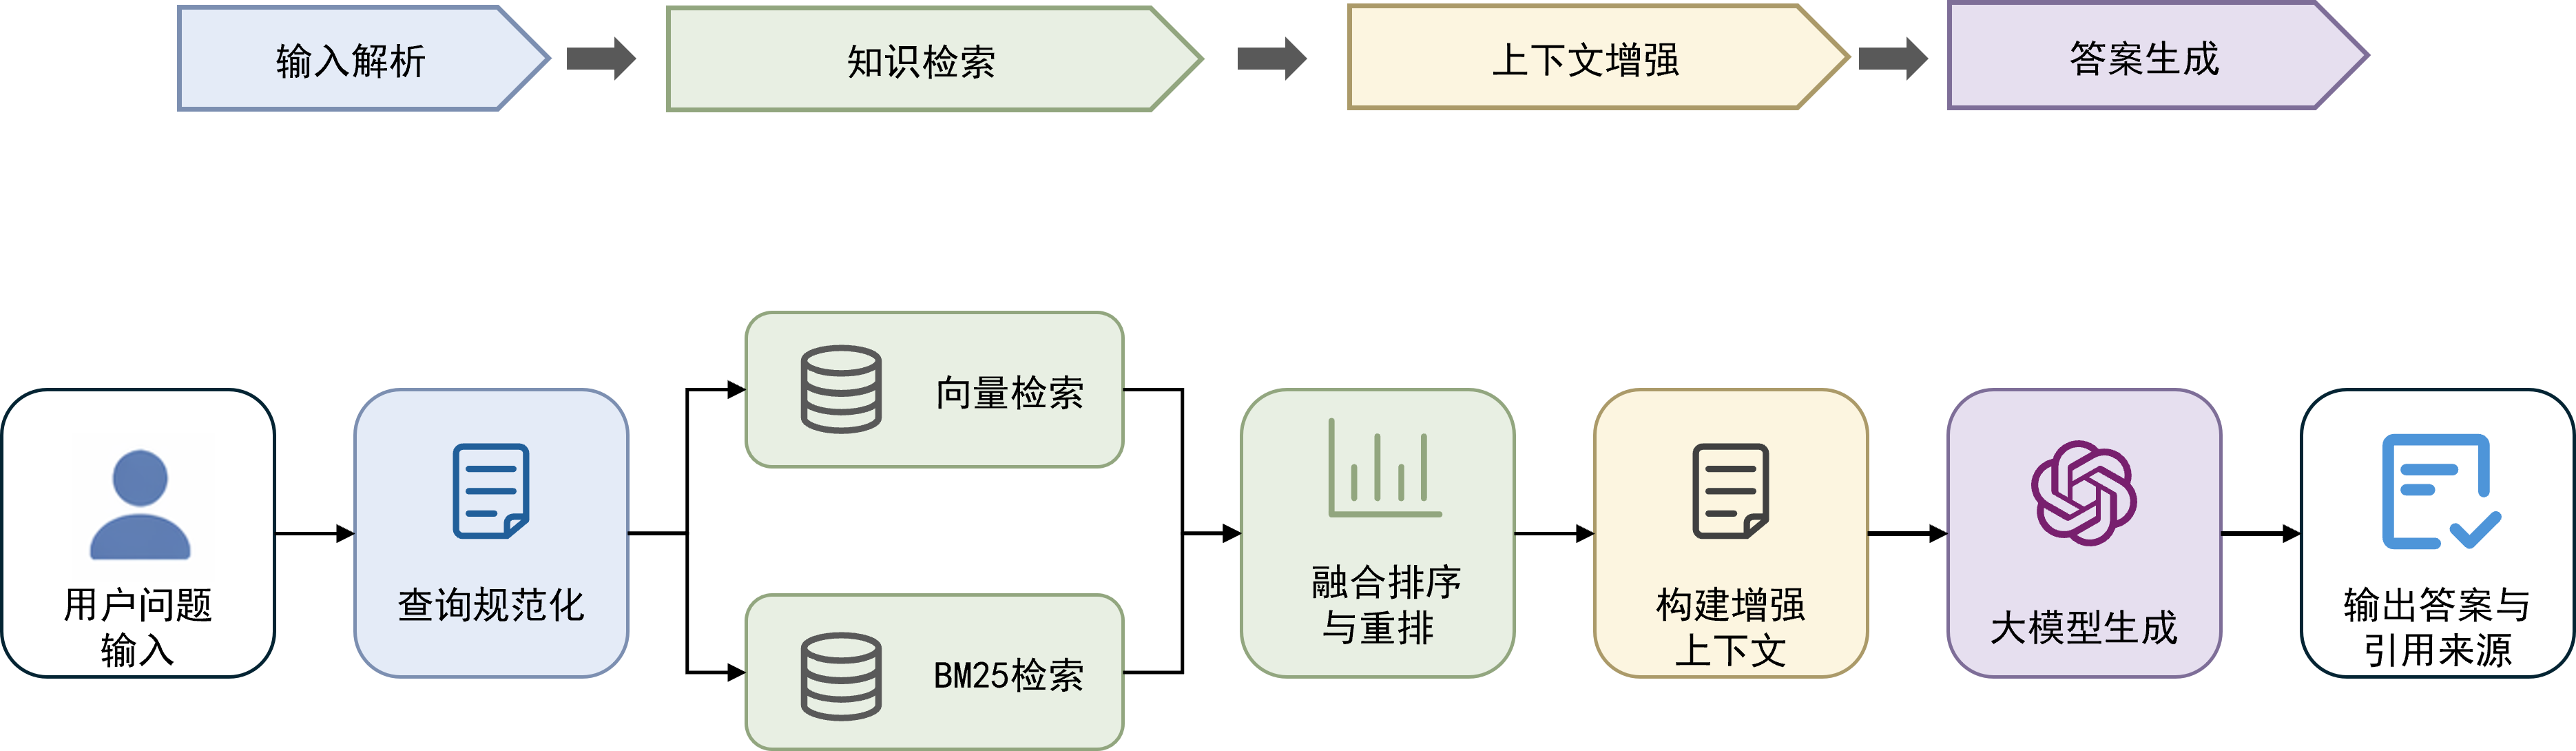
\includegraphics[width=0.8 \textwidth]{image/4/framework.png}
    \caption{系统流程图}
    \label{fig:system-flowchart}
\end{figure}

在输入解析阶段，系统会先接收用户发来的自然语言问句，再结合之前几轮对话的历史信息对查询做语义补全和规范化处理，从而让后续检索能更精准地锁定用户真正的意图。

在知识检索阶段，系统采用混合检索策略，一路是基于向量的语义检索，它依靠Embedding模型把文本映射到高维的向量空间中来表示语义、捕捉深层的语义相似性；另一路则是基于关键词的BM25检索，专门负责精确锁定关键字上的匹配，特别针对于医学领域海量的专业术语。如果只依赖向量检索，有可能会漏掉或误判某些关键医学名词，于是把BM25作为补充手段能有效提高整个检索结果的准确度和覆盖面，两路结果检索完成之后，系统再经过融合、排序和重排这几道处理，筛选出最相关的一批文本片段。

在上下文增强阶段，系统将上一阶段筛选出的文本片段，用户问题和对话历史，通过事先设计好的prompt模板结合，构建成一份结构清晰的输入，让模型在阅读时能轻易分辨出哪一部分来自使用者的提问、哪一部分是从知识库里调出来的参考资料。

在答案生成阶段，模型依据这份组合好的输入来产出回答，以流式方式逐字输出。在生成全部完成后，系统会把检索到的文献信息返还给用户当成参考，同时也会记录下这次输入和输出所消耗的token数量，后者将会跟对话历史一同保存进数据库，为下一次用户提问时构建多轮对话上下文时估算长度提供依据。

\section{业务层实现}

业务层后端服务基于Node.js的框架Express开发，负责用户身份认证与权限控制、会话管理、消息持久化、模型服务编排与知识库运维接口。

\subsection{后端服务架构设计}

系统后端入口位于统一应用服务中，主要路由模块包括用户认证、会话管理、消息管理、模型调用和知识库管理。各模块职责如下：
\begin{enumerate}[label =(\arabic*)]

    \item 认证模块：提供注册与登录接口，完成密码加密与令牌签发；
    \item 会话模块：管理会话创建、查询、更新与软删除；
    \item 消息模块：管理消息读写与 token 信息回填；
    \item 模型模块：接收问题请求，调用本地模型服务并返回生成结果；
    \item 知识库模块：提供文档元信息管理、索引状态查询与重建能力。

\end{enumerate}

\subsection{会话管理}

会话管理是后端业务逻辑中的核心部分。系统为每个用户维护独立会话空间，并将每轮对话中的角色、正文、时间戳、引用证据和统计信息写入数据库，以支撑历史记录查询和多轮上下文组织。

在具体流程上，当用户提交问题时，后端会先判断当前会话是否存在；若不存在，则创建新会话并写入用户消息；若已存在，则直接在原会话下追加消息。模型返回回答后，系统再将助手回答与证据一并写回，并同步更新会话摘要和更新时间。这样既能保证多轮对话连续性，也方便前端展示最近会话状态。

\subsection{数据库}

后端数据库使用PostgreSQL，PostgreSQL可支持使用“JSONB内容字段”的存储。在保存用户与模型的对话历史时，用户消息和模型消息、系统消息的结构并不完全相同，例如：模型消息在返回时会携带RAG过程中检索到的资料信息，而用户消息则不需要这个字段。面对这类字段需求参差不齐的情况，JSONB 格式比常规的关系型表设计要灵活得多，能很好地应对问答消息里字段不固定、结构可能时常变动的状况。系统将用户、会话、消息等较为固定的实体信息保存在关系型字段里；将消息正文、引用资料信息、Token消耗等可选字段的内容存放在JSONB字段中。通过这一混合存储方式，就能用同一张表适应模型消息和用户消息的不同格式，不必再去为每一种消息单独建表，或在一张表中留下大量的空字段。  

表\ref{tab:backend-core-tables}中列出了系统中关键的数据表及其主要字段，其中，users表用于存储用户信息，并且为每个用户分配独特的id，用户id是对其他表查询的关键信息；conversations表用于存储会话元信息（标题、更新时间、软删除标记等）；messages表用于保存逐轮对话内容与token统计信息；medical\_documents表用于保存知识文档元数据；knowledge\_index\_meta表用于记录索引状态（dirty/running/synced/error）。

\begin{table}[htbp]
    \centering
    \caption{后端核心数据表}
    
    \setlength{\tabcolsep}{8pt} % 列间距（原来14mm太大了）
    
    \begin{tabular}{l c p{5cm}} % 第三列自动换行
        \toprule
        数据表名 & 核心字段 & 作用 \\
        \midrule
        user & id, password\_hash, is\_admin & 用户身份与权限管理 \\
        conversations & user\_id, title, last\_message, is\_deleted & 会话元信息管理 \\
        messages & conversation\_id, role, content, tokens & 多轮消息与 token 信息存储 \\
        medical\_documents  &  title, source, ingest\_key, tags &  知识文档元信息维护 \\
        knowledge\_index\_meta  &  status, last\_reindexed\_at, last\_error  &  索引状态追踪与运维监控 \\
        \bottomrule
    \end{tabular}
    \label{tab:backend-core-tables}
\end{table}

\subsection{流式转发}

为了缩短用户等待时的空白感，后端加入了面向前端的流式转发机制，Node.js服务接收到模型服务返回的增量文本后，会继续通过SSE把内容持续发送到前端，这样回答还没有完全生成时，界面上就已经能看到文本逐步显示出来，整体交互会更连贯。

具体处理时，后端会先把用户消息和助手占位消息写入数据库，再和模型服务建立流式连接，后续只要模型服务持续返回新的文本片段，后端就会把这些内容整理成前端可以解析的事件数据并立即转发出去；等回答生成结束后，再统一回写完整结果和相关统计信息，这样一来，界面能够及时更新，数据库里保存的内容也能保持完整一致。

\subsection{知识库管理接口}

知识库管理接口主要面向管理员使用，任务是把文档维护和索引管理这一类后台操作组织起来，接口内容包括文档元信息查询、文本上传入库、索引状态查看、增量更新和全量重建等，这样知识库相关操作就能放在统一入口中处理，管理起来也更方便。

在知识入库过程中，后端接收到文本内容和来源信息后，会继续调用后续处理流程，依次完成文本清洗、内容切分、Embedding编码和索引写入，写入成功以后，再触发模型服务对索引进行热更新；如果中间某个环节出现问题，系统会把错误状态记录下来，并返回较明确的提示信息，方便后面排查和恢复，这样处理之后，知识更新就不再是彼此分散的单独步骤，而是能和在线问答过程更自然地衔接起来。

\section{模型与RAG服务实现}

\subsection{模型服务功能设计}

本文将模型推理部分独立部署为Python服务，并和业务后端解耦。这样设计有两点直接好处，一是可以把GPU资源集中用于检索和推理任务，减少和业务逻辑混合部署带来的资源竞争，二是后续即使替换Embedding模型、重排模型或生成模型版本，也不需要同步改动业务层接口。

在职责划分上，模型服务主要承担四类任务，一是接收业务层转发的问题、历史对话和生成参数，二是完成查询向量化、候选召回和重排，输出可供生成阶段使用的证据集合，三是按照提示词模板把问题、历史消息和检索证据组织成统一输入，再调用生成模型产出回答，四是以同步或流式方式把结果返回业务层，同时附带引用证据和必要状态信息。经过这样的拆分后，模型服务实际上成为系统中连接“知识检索”和“回答生成”的核心执行节点。

\subsection{模型加载与推理组织}

在具体实现中，模型服务启动后会预先加载Embedding模型、重排模型和生成模型，并在内存中保持可复用状态，减少重复初始化带来的时间开销。生成模型部分采用“基础模型 + 适配器权重”的组织方式，基础模型负责通用语言生成，DPO训练得到的适配器权重在加载后参与实际推理，用于改善医学场景下的回答风格、风险提示和边界控制能力。这种组织方式既保留了基础模型的通用表达能力，也便于后续持续迭代微调权重。

在推理流程上，模型服务不是接收问题后直接生成回答，而是按固定顺序执行“检索准备、候选筛选、上下文构建、模型生成”四个步骤。服务先根据用户问题构造检索查询，再调用检索与重排模块得到排序后的证据片段，随后把问题、历史消息和证据封装成模型输入，最后调用生成模型输出回答。通过这种流程化组织，模型服务能够把第4章提出的RAG方法和DPO优化能力稳定地落实到在线推理过程中。

\subsection{接口设计与结果返回}

为了适应不同交互场景，模型服务对外提供同步调用和流式调用两类接口。同步接口更适合调试、批量测试和非实时任务，调用方在一次请求中等待完整回答返回；流式接口更适合在线问答场景，模型服务会把回答拆成连续文本片段逐步输出，让前端能够边接收边展示，减少等待完整回答时的停顿感。

在返回内容上，模型服务不只输出最终回答文本，还会同时返回检索证据、引用来源和必要状态字段。对于流式模式，服务通过事件形式持续返回增量内容，并在结束时统一发送完成标记；如果推理过程中出现异常，则返回错误事件并附带错误信息，便于业务层捕获和提示。通过这种接口设计，模型服务向上对接业务后端时可以保持调用方式统一，向下也能兼容不同推理模式。

\subsection{RAG请求编排流程}

在线问答请求到达后，业务后端会先完成会话识别、历史消息提取和参数整理，再把当前问题、必要上下文和调用配置转发给模型服务。模型服务收到请求后，按预设顺序依次执行查询规范化、候选召回、结果筛选、上下文构造和回答生成，最后把完整结果回传给业务层。

这种编排方式的特点在于，RAG链路不是单一函数调用，而是一条由多个步骤组成的服务流程。每个步骤都有相对明确的输入和输出，例如召回阶段输出候选文本集合，重排阶段输出重新排序后的证据列表，上下文构建阶段输出可直接送入生成模型的结构化输入。通过这种分阶段组织，系统可以在不中断整体服务的前提下，对单个环节进行调试、替换和性能优化。

\subsection{检索链路调度}

在工程实现上，RAG服务通过统一调度入口管理检索相关步骤。系统不会把BM25检索、向量检索、融合排序和重排分别暴露为分散接口，而是由模型服务在内部完成链路编排，对外只表现为一次“检索增强问答”调用。这样设计可以减少业务层对底层检索细节的依赖，后续即使调整召回方式或更换重排模型，上层接口也不需要同步修改。

在调度过程中，系统先根据用户问题生成检索查询，再并行触发不同召回路径，随后对候选结果做统一编号、去重和排序。完成排序后，系统只保留数量受控的高相关证据进入下游生成流程，避免把大量低价值文本直接送入模型。也就是说，RAG服务在系统中的作用不只是“把资料找出来”，更重要的是在有限上下文窗口内尽可能选出最值得保留的证据。

\subsection{证据封装与结果回传}

完成检索和筛选后，RAG服务还需要把中间结果转换成适合业务层和前端使用的结构。为此，系统会把最终证据统一封装成结构化对象，其中包含文本内容、来源信息、标题路径、相关性顺序和必要标识字段。这样处理后，生成模型可以直接使用这些证据构造输入，业务后端也可以在回答完成后把同一份证据回写数据库，前端则能基于这些字段展示“引用来源”或“检索依据”等信息。

在结果返回阶段，RAG服务输出的不只是最终回答文本，还包括检索证据、引用元数据和必要状态字段。对系统来说，这一点很关键，因为医学问答不仅需要给出结论，还需要在工程上支持结果追溯。把检索证据和生成结果作为同一次调用的组成部分统一返回后，系统就能保持“回答内容”和“回答依据”之间的一致性。

\subsection{索引更新与一致性维护}

RAG服务的另一个关键实现点，是知识更新后的索引一致性维护。由于知识库内容不是静态不变的，系统在管理员新增、修改或删除文档后，需要重新执行文本切分、向量编码和索引写入等步骤。为了避免知识内容已经更新而检索结果仍停留在旧状态，系统在知识库管理接口和RAG服务之间建立了索引状态联动机制，当文档发生变化时，会同步更新索引状态标记，并在必要时触发增量更新或全量重建流程。

这样的设计使RAG服务不仅负责在线问答时的实时检索，也承担了知识检索能力持续可用的维护职责。只有索引状态、文档内容和在线服务三者保持一致，RAG系统才能在真实应用中稳定运行。因此，RAG服务工程实现的重点在于检索增强链路如何被稳定组织、如何与业务层协同、以及如何支持后续运维更新。

\section{前端实现}

\subsection{前端UI架构与路由设计}

前端界面采用React构建，并结合路由机制完成页面切换，整体上分为登录页、注册页、问答主页和知识库管理页，不同页面各自承担明确任务，这样既方便功能拆分，也有利于后续继续补充新模块。登录和注册页面主要处理身份验证，问答主页负责会话列表、消息展示和问题输入，知识库管理页则面向管理员，用来处理文档维护与索引相关操作。

在界面组织上，前端把通用能力拆分到页面、组件和Hook三个层次，页面负责整体布局和功能组合，组件负责消息列表、输入框、侧边栏等可复用界面，Hook负责会话状态、消息请求和交互流程管理，这种划分方式能让界面结构更清楚，代码之间的联系也更容易梳理。主页部分采用侧边栏与主内容区的布局，侧边栏用于展示历史会话和常用操作，主区域用于展示问答内容与输入区域，页面层次比较直观，用户进入系统后也能较快找到对应功能。

\subsection{对话交互与流式渲染实现}

会话相关的核心逻辑集中放在自定义Hook中，发送问题时，界面会先把用户消息和助手的占位内容加入当前会话，再向后端发起流式请求，这样用户提交问题后能马上看到界面变化，等待过程也不会显得突兀。流式数据通过后端的SSE通道持续返回，前端再用ReadableStream按帧读取并解析事件，接收到delta内容后，就把新增文本接到助手回答后面，于是回答会一点点展开，形成较自然的实时反馈效果。

为了让多轮对话前后保持一致，流式输出结束后，前端还会重新拉取一次消息记录，并用后端已经保存的结果覆盖临时状态，避免在长对话过程中因为局部丢帧或上下文偏移，出现界面显示和实际数据不一致的情况；如果模型服务中途异常或连接中断，界面会直接给出明确的提示文本，使当前交互还能继续恢复，不会停在难以理解的状态里。

\subsection{消息展示与检索证据可视化}

消息展示部分支持Markdown和GFM语法渲染，因此回答中的分点说明、表格以及部分结构化内容都能较完整地显示出来，页面阅读体验也更清楚。在RAG问答场景下，系统会把检索得到的retrieved\_docs附加到助手消息中，再在回答下方用“全部引用”的折叠区域统一展示，这样答案和证据能够放在同一界面里，用户查看结论时也能顺带看到对应依据，有助于增强结果的可解释性与可追溯性。

为了减少重复信息，前端会按照source字段对引用文档进行去重，同时保留来源名称、标题层级等关键内容，便于快速核对回答依据，也便于进一步判断相关结论是否来自较可靠的医学资料，从而提高对系统输出结果的信任程度。

\section{本章小结}

本章从工程实现角度介绍了医学问答系统的整体设计。首先明确了系统在准确性、可解释性、实时性和可扩展性方面的目标；随后说明了总体架构和RAG运行流程；最后分别从后端、模型服务、RAG工程实现和前端交互四个层面展开具体实现分析。

通过上述设计与实现，本文完成了一套具备知识检索、模型生成、证据展示和会话管理能力的医学问答系统，为后续实验评估和应用验证提供了完整工程基础。
